\section{CosmoScout VR}\label{sec:cosmoscout-vr}

Cosmoscout VR is a modular, scientific, 3D visualisation of the solar system, with the goal to provide interactive,
and immersive exploration of large datasets.
Recent earth observation and space exploration in the international community has produced vast amounts of data at a
scale that can be difficult to process and visualise.

\begin{figure}[h]
    \centering
    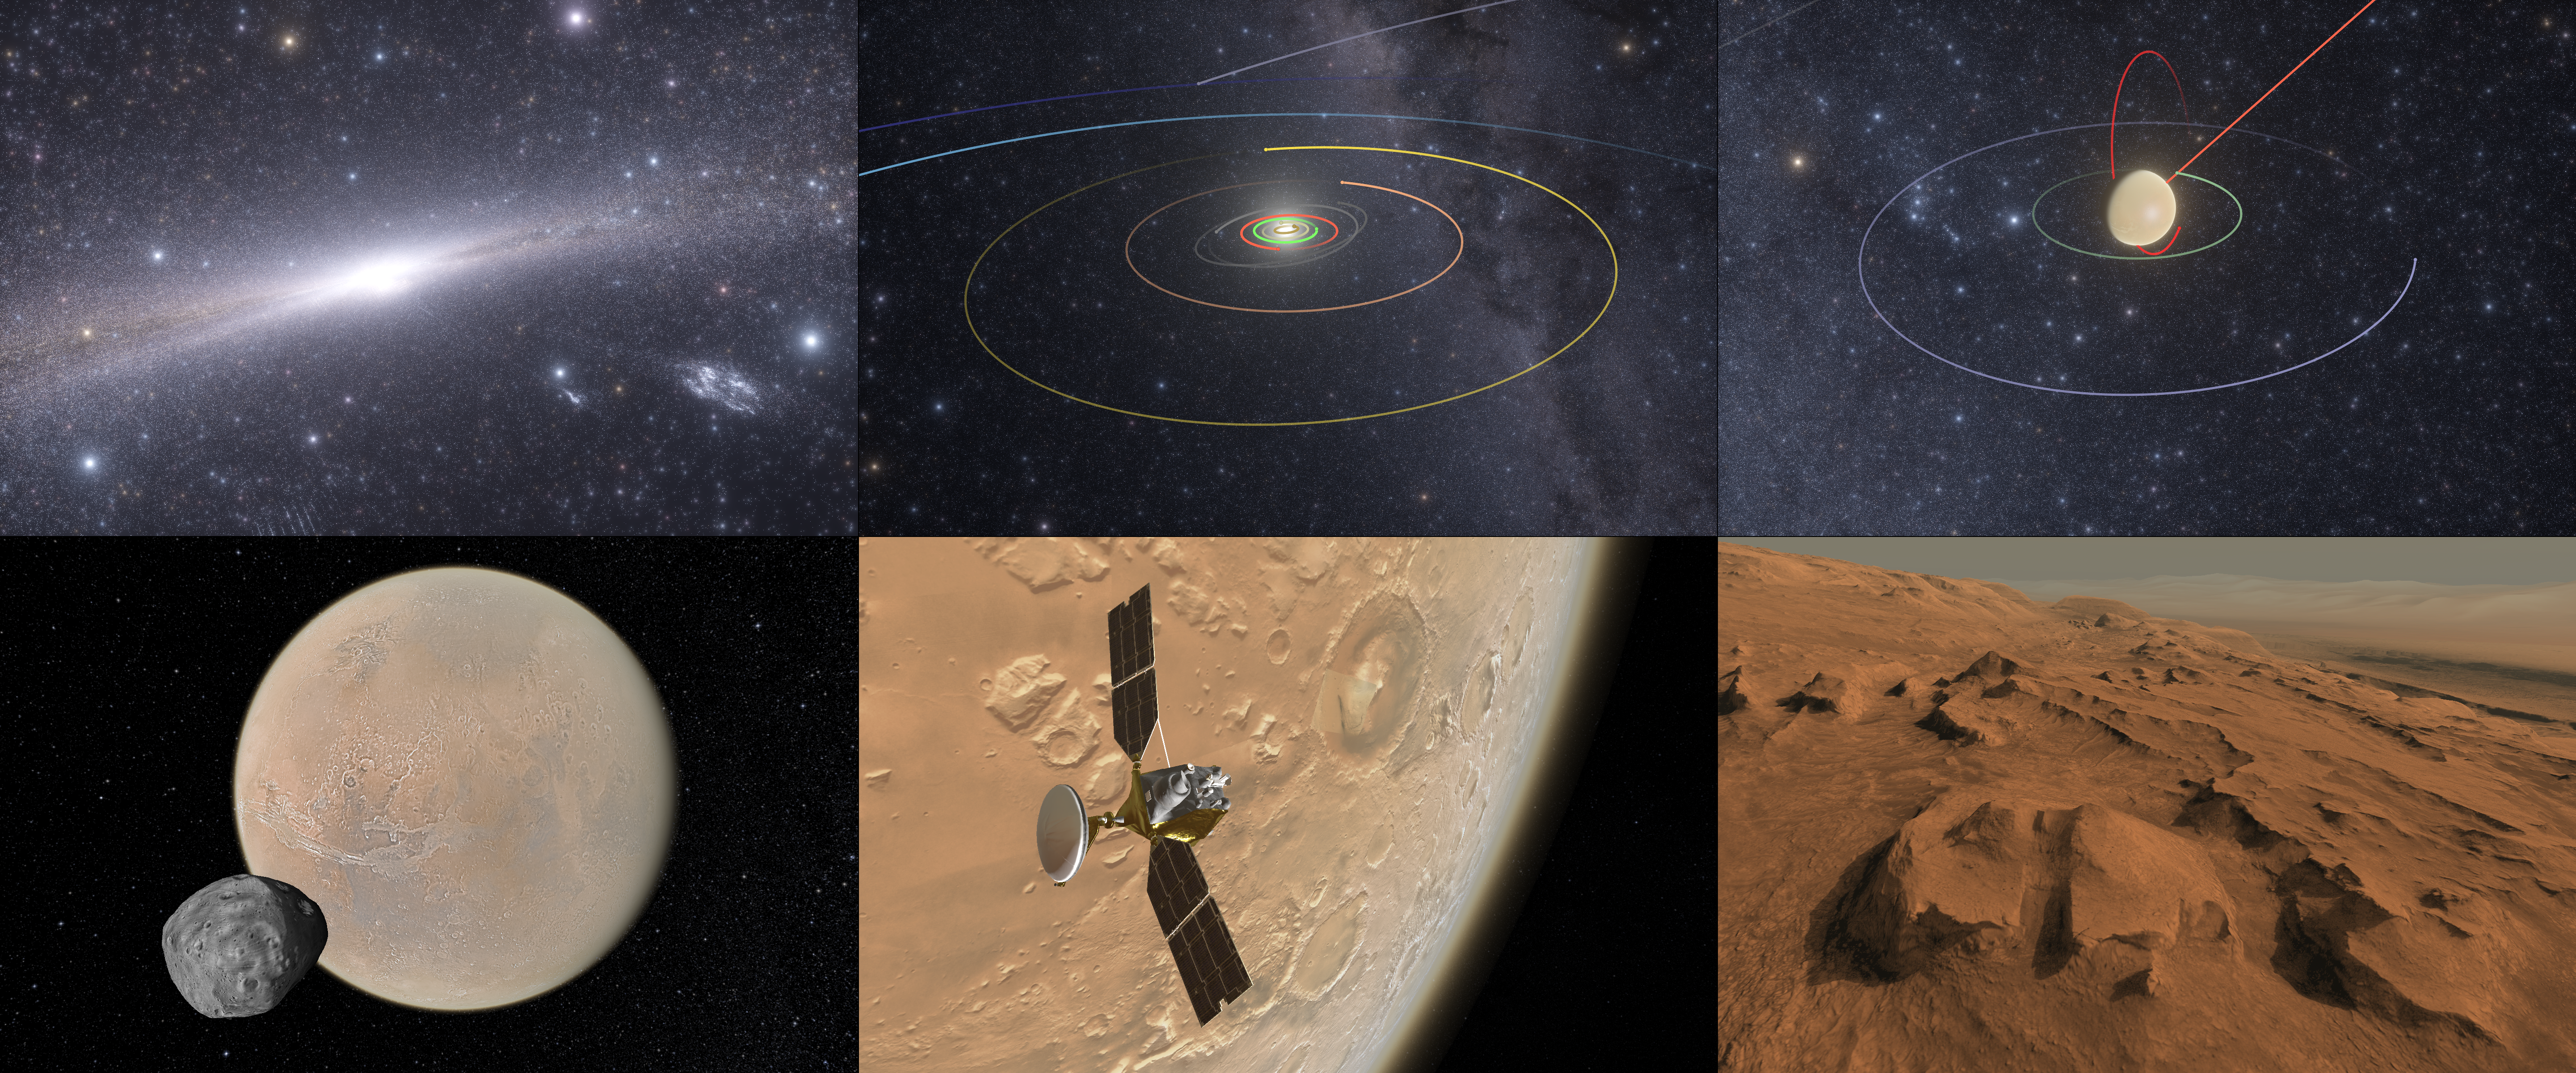
\includegraphics[width=\textwidth]{content/2_3_cosmoscout/img/cosmoscout-scales}
    \caption{Range of scale in CosmoScout VR: outer edge of the galaxy (top left), solar system overview (top center),
        overview of Mars (top right), close-up of Mars and Phobos (bottom left), close-up of the Mars Reconnaissance
        Orbiter (bottom center), and close-up of Mars surface (bottom right)~\cite{DLRmagazin2019}}
    \label{fig:cosmoscout-scales}
\end{figure}

CosmoScout VR has the goal of visualising these increasingly large datasets at diverse scales, with the virtual
environment allowing natural, and intuitive interaction, and explorative analysis of the data.
This multiscale approach tries to facilitate the seamless exploration from a street level view of a body's surface,
like examining local topography of the Mars surface, or moving around Helgoland, all the way up to examining the
solar system as a whole, and the orbits of different celestial or man-made objects around the sun, or other bodies.
Figure~\ref{fig:cosmoscout-scales} shows examples of different scales that can be used to explore data inside the
CosmoScout simulation seamlessly without interrupting the user experience.

\begin{wrapfigure}{o}{0.5\textwidth}
    \centering
    \includegraphics[width=0.5\textwidth]{content/2_3_cosmoscout/img/cosmoscout-architecture}
    \caption{CosmoScout VR architecture~\cite{CSVR}.}
    \label{fig:cosmoscout-architecture}
\end{wrapfigure}

CosmoScout VR uses a modular, layered architecture to provide high-flexibility for different use cases.
The core libraries are used in the slim executable, that is packaged with a collection of Plugins, providing
the key functionality of CosmoScout VR, while the Plugins can still be customized to focus the application for
specific use cases.
For Example, the "\textit{csp-lod-bodies}" is a Plugin enabling the drawing and fluid switching between different
level of detail for planets and moons depending on the plugins settings.
The plugin also realises a connection to a Web-Map-Services-Server over the internet to request the textures and
visualise entire planets down to a 1:1 scale, if set up and needed.
This way a multitude of different map data can be examined on different scales for a planet, and if needed the
"\textit{csp-measurement-tools}" can be loaded to provide several tools to mark locations, measure paths and
elevation lines.
Otherwise, the plugin can be left out if detailed surface mapping is not required, and the
"\textit{csp-simple-bodies}" plugin can be used in conjunction with the "\textit{csp-rings}" plugin to draw simple
textured bodies to represent the planets and their rings at a larger, less detailed scale.

The features developed in this thesis to mitigate cybersickness especially in HMD-based VR are also bundled into a
plugin, allowing the user to load the features if necessary, and ignore them if CosmoScout is used without a
VR HMD\@.

The CosmoScout base is composed of five core libraries that provide basic functionalities, using external
dependencies to realise key components.
ViSTA is used to support different devices, network synchronization, and for the scene graph.
SPICE is used in conjunction with ViSTA's scene graph for precise positioning and resource effective rendering of
celestial, and other objects at any scale, as SPICE provides a set of nested reference frames to facilitate precise
transformation of positions and orientations across a large scale, or distance within the simulation.
